%!TEX root = ../../Main.tex
\graphicspath{{Chapters/Veroboardmontering/}}
%-------------------------------------------------------------------------------

\chapter{Applikationlaget::client}

i applikationslaget bruger vi vores hovedsagelig den viden vi har lært fra opgave 7. Det vil sige vi har taget det meste af koden fra opgave 7 og modificeret den. 

Det første vi gør i koden, er at vi modtager filstørrelsen, denne bruger vi senere i koden, og bruger den itl at tjekke om filen eksisterer, dette gør vi på den måde at hvis file size er 0, eksisterer filen ikke. 

Herefter laver vi en file descriptor, som peger på filen, den bruger vi til at kunne åbne filen. Hvis file descriptoreren er -1, har vi modtaget noget corrupt, og vi kører derfor en error på den. 

Hvis der ikke er overført korrupt data, modtager vi herefter filen, med 100 bytes af gangen, når der ikke er mere end 1000 bytes tilbage sender vi en "last bytes recieved" og udkriver størrelsen på arrayet. 

\begin{lstlisting}[frame=single]  % Start your code-block

void file_client::receiveFile (std::string fileName, Transport::Transport *myTransport)
{
    char buffer[BUFSIZE] = {0};
    int n, recievedSize = 0;
    long fsize;
    int fd;

    /*Filstoerrelse*/
    myTransport->receive(buffer,BUFSIZE);
    fsize = atol(buffer);
    printf("Fil stoerrelse: %d \n", fsize);

    if (fsize == 0)
    {
        fprintf(stderr,"ERROR: Filen findes ikke. \n");
        exit(0);
    }

    /*Laver file descriptor*/
    fd = open(fileName.c_str(), O_WRONLY | O_CREAT,S_IXGRP);
    if (fd == -1) error ("Kunne ikke aabne fil");
    printf("File descriptor: %d \n", fd);

    /*Fil fra serveren*/
    for (int i = 0; i<fsize/BUFSIZE+1; i++)
    {

        if (i<fsize/BUFSIZE) //Hvis der er mere end 1000bit tilbage
        {
            recievedSize = myTransport->receive(buffer,BUFSIZE);
            n = write(fd, buffer, BUFSIZE); /*fil bliver lagt over i fd*/

        }

        else
        {
            recievedSize = myTransport->receive(buffer,fsize%BUFSIZE);
            n = write(fd, buffer, fsize%BUFSIZE); /*fil bliver lagt over i fd*/

            printf("Sidste bit er modtaget: %d \n", recievedSize);

        }


    }

    close(fd);
}

\end{lstlisting}	


\begin{figure}[H]
\centering
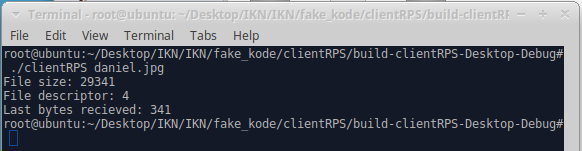
\includegraphics[width = 300 pt]{Img/client_recieve.PNG}
\caption{Client modtager fil}
\label{fig:konceptbillede}
\end{figure}
